% Generated by make_fig_pdg.py from programs/*.py and the study's code. Do not edit by hand.
\documentclass[border=2pt]{standalone}
\usepackage[T1]{fontenc}\usepackage{newtxtext,newtxmath}\usepackage[varqu,scaled=0.95]{zi4}
\usepackage{amsmath,xcolor,listings,tikz}\usetikzlibrary{arrows.meta,calc}
\definecolor{cblue}{HTML}{0072B2}\definecolor{cver}{HTML}{D55E00}\definecolor{cgreen}{HTML}{009E73}
\definecolor{cpurple}{HTML}{7E57C2}
\lstdefinestyle{qiskit}{language=Python,basicstyle=\ttfamily\fontsize{5.6}{6.9}\selectfont,numbers=left,
  numberstyle=\fontsize{5}{6}\selectfont\color{black!55},numbersep=3pt,keywordstyle=\color{cblue}\bfseries,
  commentstyle=\color{black!55}\itshape,showstringspaces=false,frame=single,rulecolor=\color{black!25},
  xleftmargin=13pt,framexleftmargin=11pt,framerule=0.4pt,columns=flexible,keepspaces=true,aboveskip=0pt,belowskip=0pt}
\tikzset{
  op/.style={rectangle, rounded corners=2pt, draw=black!60, line width=0.45pt, fill=white, align=center,
             inner xsep=2pt, inner ysep=1.3pt, font=\ttfamily\fontsize{6}{6.6}\selectfont},
  insl/.style={op, fill=cblue!22},
  missdep/.style={op, draw=cver, line width=0.9pt, dash pattern=on 1.6pt off 1pt},
  missdepsl/.style={missdep, fill=cblue!22},
  entx/.style={op, fill=cpurple!30, draw=cpurple, line width=0.8pt},
  lvdu/.style={op, fill=cblue!58},
  lvcp/.style={op, fill=cblue!32},
  lvqd/.style={op, fill=cblue!11, draw=cblue!80!black},
  clq/.style={cl, fill=black!14, draw=black!60},
  cpdgE/.style={-{Stealth[length=1.2mm]}, draw=black!55, line width=0.5pt, dash pattern=on 0.6pt off 0.9pt},
  crit/.style={double=white, double distance=0.7pt, line width=0.5pt},
  dataE/.style={-{Stealth[length=1.2mm]}, draw=black!50, line width=0.45pt},
  quantumE/.style={-{Stealth[length=1.4mm]}, draw=cblue, line width=1.1pt},
  controlE/.style={-{Stealth[length=1.3mm]}, draw=cgreen, line width=0.85pt, dash pattern=on 2.2pt off 1.1pt},
  missingE/.style={-{Stealth[length=1.3mm]}, draw=cver, line width=0.85pt, dash pattern=on 1.8pt off 1.2pt},
  ttl/.style={font=\footnotesize\bfseries, anchor=south},
  cl/.style={op, draw=black!45, fill=black!4, font=\ttfamily\fontsize{5.6}{6.2}\selectfont},
  clsl/.style={cl, fill=cblue!22, draw=black!60},
  loopbox/.style={draw=black!40, rounded corners=3pt, line width=0.5pt, dash pattern=on 2.5pt off 1.2pt},
  boxlbl/.style={font=\ttfamily\fontsize{5.2}{5.6}\selectfont, text=black!65, inner sep=1pt},
  note/.style={font=\scriptsize, anchor=north, align=center},
}
\begin{document}
\begin{minipage}{17.8cm}\begin{minipage}[t]{5.5cm}\vspace{0pt}{\footnotesize\textbf{(a) VQE ansatz}}\\[3pt]\lstinputlisting[style=qiskit,firstline=4,lastline=20,firstnumber=4]{programs/_display/ansatz.py}\end{minipage}\hfill\begin{minipage}[t]{12.2cm}\vspace{0pt}\centering{\footnotesize\textbf{(b) Dependence graph of the four rules, criterion $q_0$}}\\[4pt]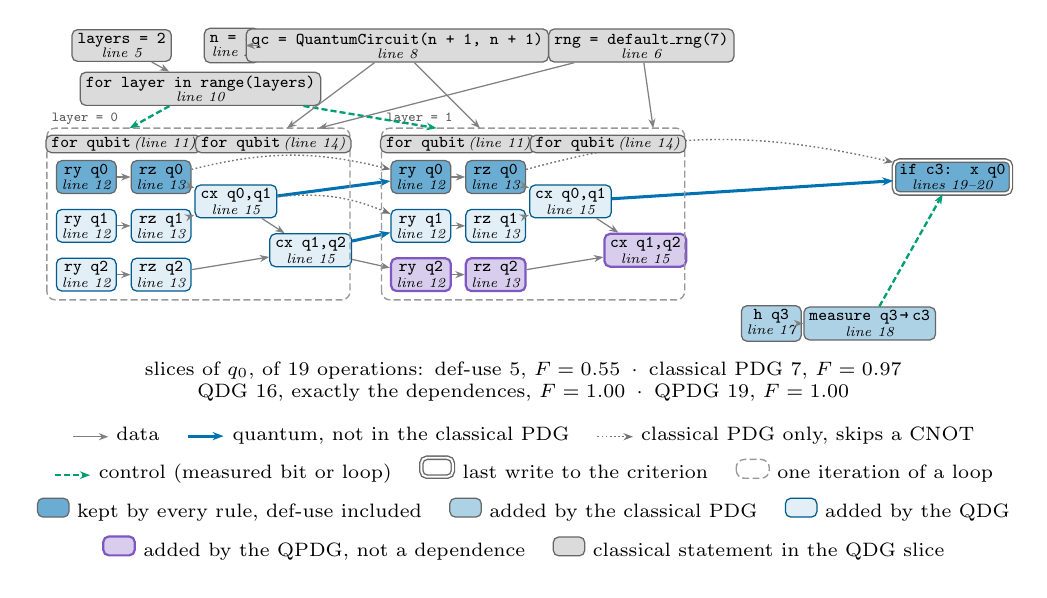
\begin{tikzpicture}
\node[lvdu] (m0) at (0.000,0.000) {ry q0\\[-1pt]{\rmfamily\itshape\fontsize{5}{5.5}\selectfont line 12}};
\node[lvdu] (m1) at (0.950,0.000) {rz q0\\[-1pt]{\rmfamily\itshape\fontsize{5}{5.5}\selectfont line 13}};
\node[lvqd] (m2) at (0.000,-0.620) {ry q1\\[-1pt]{\rmfamily\itshape\fontsize{5}{5.5}\selectfont line 12}};
\node[lvqd] (m3) at (0.950,-0.620) {rz q1\\[-1pt]{\rmfamily\itshape\fontsize{5}{5.5}\selectfont line 13}};
\node[lvqd] (m4) at (0.000,-1.240) {ry q2\\[-1pt]{\rmfamily\itshape\fontsize{5}{5.5}\selectfont line 12}};
\node[lvqd] (m5) at (0.950,-1.240) {rz q2\\[-1pt]{\rmfamily\itshape\fontsize{5}{5.5}\selectfont line 13}};
\node[lvqd] (m6) at (1.900,-0.310) {cx q0,q1\\[-1pt]{\rmfamily\itshape\fontsize{5}{5.5}\selectfont line 15}};
\node[lvqd] (m7) at (2.850,-0.930) {cx q1,q2\\[-1pt]{\rmfamily\itshape\fontsize{5}{5.5}\selectfont line 15}};
\node[lvdu] (m8) at (4.250,0.000) {ry q0\\[-1pt]{\rmfamily\itshape\fontsize{5}{5.5}\selectfont line 12}};
\node[lvdu] (m9) at (5.200,0.000) {rz q0\\[-1pt]{\rmfamily\itshape\fontsize{5}{5.5}\selectfont line 13}};
\node[lvqd] (m10) at (4.250,-0.620) {ry q1\\[-1pt]{\rmfamily\itshape\fontsize{5}{5.5}\selectfont line 12}};
\node[lvqd] (m11) at (5.200,-0.620) {rz q1\\[-1pt]{\rmfamily\itshape\fontsize{5}{5.5}\selectfont line 13}};
\node[entx] (m12) at (4.250,-1.240) {ry q2\\[-1pt]{\rmfamily\itshape\fontsize{5}{5.5}\selectfont line 12}};
\node[entx] (m13) at (5.200,-1.240) {rz q2\\[-1pt]{\rmfamily\itshape\fontsize{5}{5.5}\selectfont line 13}};
\node[lvqd] (m14) at (6.150,-0.310) {cx q0,q1\\[-1pt]{\rmfamily\itshape\fontsize{5}{5.5}\selectfont line 15}};
\node[entx] (m15) at (7.100,-0.930) {cx q1,q2\\[-1pt]{\rmfamily\itshape\fontsize{5}{5.5}\selectfont line 15}};
\node[lvcp] (m16) at (8.700,-1.860) {h q3\\[-1pt]{\rmfamily\itshape\fontsize{5}{5.5}\selectfont line 17}};
\node[lvcp] (m17) at (9.950,-1.860) {measure q3\,\textrightarrow\,c3\\[-1pt]{\rmfamily\itshape\fontsize{5}{5.5}\selectfont line 18}};
\node[lvdu,crit] (m18) at (11.000,0.000) {if c3: x q0\\[-1pt]{\rmfamily\itshape\fontsize{5}{5.5}\selectfont lines 19--20}};
\draw[dataE] (m0) -- (m1);
\draw[dataE] (m1) -- (m6);
\draw[dataE] (m2) -- (m3);
\draw[dataE] (m3) -- (m6);
\draw[dataE] (m4) -- (m5);
\draw[dataE] (m5) -- (m7);
\draw[dataE] (m6) -- (m7);
\draw[quantumE] (m6) -- (m8);
\draw[quantumE] (m7) -- (m10);
\draw[dataE] (m7) -- (m12);
\draw[dataE] (m8) -- (m9);
\draw[dataE] (m9) -- (m14);
\draw[dataE] (m10) -- (m11);
\draw[dataE] (m11) -- (m14);
\draw[dataE] (m12) -- (m13);
\draw[dataE] (m13) -- (m15);
\draw[dataE] (m14) -- (m15);
\draw[quantumE] (m14) -- (m18);
\draw[dataE] (m16) -- (m17);
\draw[controlE] (m17) -- (m18);
\draw[cpdgE] (m1) to[bend left=14] (m8);
\draw[cpdgE] (m6) to[bend left=14] (m10);
\draw[cpdgE] (m9) to[bend left=14] (m18);
\draw[loopbox] (-0.500,-1.560) rectangle (3.350,0.620);
\node[boxlbl, anchor=south west] at (-0.480,0.630) {layer = 0};
\node[clq, inner ysep=0.6pt] at (0.475,0.420) {for qubit\,{\rmfamily\itshape\fontsize{5}{5.5}\selectfont (line 11)}};
\node[clq, inner ysep=0.6pt] at (2.375,0.420) {for qubit\,{\rmfamily\itshape\fontsize{5}{5.5}\selectfont (line 14)}};
\draw[loopbox] (3.750,-1.560) rectangle (7.600,0.620);
\node[boxlbl, anchor=south west] at (3.770,0.630) {layer = 1};
\node[clq, inner ysep=0.6pt] at (4.725,0.420) {for qubit\,{\rmfamily\itshape\fontsize{5}{5.5}\selectfont (line 11)}};
\node[clq, inner ysep=0.6pt] at (6.625,0.420) {for qubit\,{\rmfamily\itshape\fontsize{5}{5.5}\selectfont (line 14)}};
\node[clq] (cly) at (0.450,1.670) {layers = 2\\[-1pt]{\rmfamily\itshape\fontsize{5}{5.5}\selectfont line 5}};
\node[clq] (cn) at (1.850,1.670) {n = 3\\[-1pt]{\rmfamily\itshape\fontsize{5}{5.5}\selectfont line 4}};
\node[clq] (cqc) at (3.950,1.670) {qc = QuantumCircuit(n + 1, n + 1)\\[-1pt]{\rmfamily\itshape\fontsize{5}{5.5}\selectfont line 8}};
\node[clq] (crng) at (7.050,1.670) {rng = default\_rng(7)\\[-1pt]{\rmfamily\itshape\fontsize{5}{5.5}\selectfont line 6}};
\node[clq] (cfor) at (1.450,1.120) {for layer in range(layers)\\[-1pt]{\rmfamily\itshape\fontsize{5}{5.5}\selectfont line 10}};
\draw[dataE] (cn) -- (cqc);
\draw[dataE] (cly) -- (cfor);
\draw[controlE] (cfor) -- (0.550,0.620);
\draw[controlE] (cfor) -- (4.450,0.620);
\draw[dataE] (cqc) -- (2.550,0.620);
\draw[dataE] (cqc) -- (5.000,0.620);
\draw[dataE] (crng) -- (2.950,0.620);
\draw[dataE] (crng) -- (7.200,0.620);
\node[font=\scriptsize, anchor=north, align=center] (note) at (5.550,-2.220) {slices of $q_0$, of 19 operations:\enspace def-use 5, $F = 0.55$\enspace$\cdot$\enspace classical PDG 7, $F = 0.97$\\QDG 16, exactly the dependences, $F = 1.00$\enspace$\cdot$\enspace{}QPDG 19, $F = 1.00$};
\node[anchor=north, align=center] at ($(note.south)+(0,-0.08)$) {{\scriptsize \mbox{\tikz\draw[dataE](0,0)--(0.45,0); data}\hspace{0.9em} \mbox{\tikz\draw[quantumE](0,0)--(0.45,0); quantum, not in the classical PDG}\hspace{0.9em} \mbox{\tikz\draw[cpdgE](0,0)--(0.45,0); classical PDG only, skips a CNOT}}\\[2pt]{\scriptsize \mbox{\tikz\draw[controlE](0,0)--(0.45,0); control (measured bit or loop)}\hspace{0.9em} \mbox{\tikz\node[op,crit,minimum width=4mm,minimum height=2.4mm]{}; last write to the criterion}\hspace{0.9em} \mbox{\tikz\draw[loopbox](0,0)rectangle(0.42,0.24); one iteration of a loop}}\\[2pt]{\scriptsize \mbox{\tikz\node[lvdu,minimum width=4mm,minimum height=2.4mm]{}; kept by every rule, def-use included}\hspace{0.9em} \mbox{\tikz\node[lvcp,minimum width=4mm,minimum height=2.4mm]{}; added by the classical PDG}\hspace{0.9em} \mbox{\tikz\node[lvqd,minimum width=4mm,minimum height=2.4mm]{}; added by the QDG}}\\[2pt]{\scriptsize \mbox{\tikz\node[entx,minimum width=4mm,minimum height=2.4mm]{}; added by the QPDG, not a dependence}\hspace{0.9em} \mbox{\tikz\node[clq,minimum width=4mm,minimum height=2.4mm]{}; classical statement in the QDG slice}}};
\end{tikzpicture}\end{minipage}\end{minipage}\end{document}
